\chapter{Creating content}

\section{Creating a basic page}

In the previous chapter we learned how to create a content type. In this chapter we will learn how to create the content itself. An instance of a content type (a.k.a. a piece of content) is called a \textbf{Node} in Drupal. Creating content is easy, just go to \textbf{Content $\rightarrow$ Add content}. On this page you will see an overview of the different content types (Figure \ref{fig:add_content_content_types})


  \begin{figure}[H]
  	\centering
  	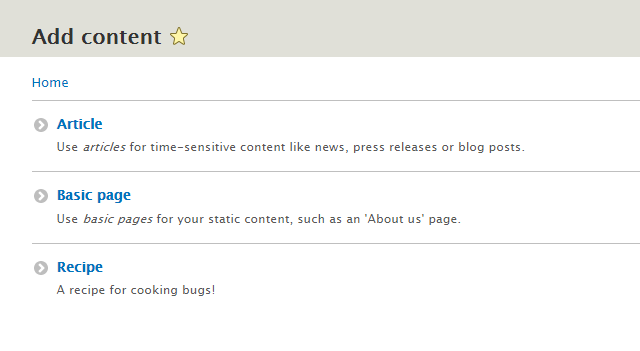
\includegraphics[width=\textwidth]{chapter5/add_content_content_types}
  	\caption{Add content, overview content types}
  	\label{fig:add_content_content_types}
  \end{figure}
  
  We are going to add a basic page. This page will explain why it is good to eat bugs. Go to \textbf{Content $\rightarrow$ Add content $\rightarrow$ Basic page}. Use the following settings: 
  
  \begin{description}
  	\item[Title] Why bugs
  	\item[Body] See file \url{chapter5/reasons to eat bugs.txt} included in the course attachments.
  \end{description}
  
  On the right side you have several menu items. These allow you to change your posts properties. Under \textbf{Menu settings} add a menu link to the \textbf{Main navigation} (figure \ref{fig:bitingbugs_publishing_options_basic_page})
  
  \begin{figure}[H]
  	\centering
  	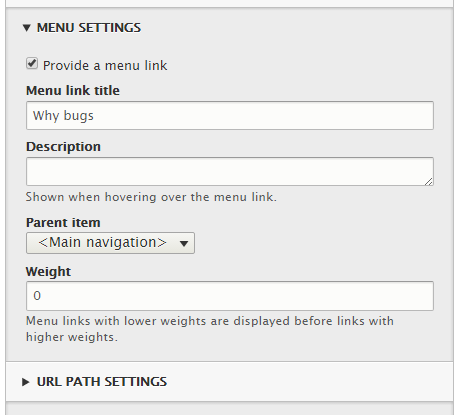
\includegraphics[width=\textwidth]{chapter5/bitingbugs_publishing_options_basic_page}
  	\caption{Basic page publishing options}
  	\label{fig:bitingbugs_publishing_options_basic_page}
  \end{figure}
  
  Click \textbf{Save and publish}
  
  \section{Creating a recipe}
  
  Go to \textbf{Content $\rightarrow$ Add content $\rightarrow$ Recipe}. Figure \ref{fig:bitingbugs_create_recipe_problem} shows the editing page for our recipe. As you can see we have a \textbf{Name} and \textbf{Title} element. We don't need the title element. Remove it by going to: \textbf{Structure $\rightarrow$ Content types $\rightarrow$ Recipe $\rightarrow$ Manage fields $\rightarrow$ Manage form display}. Move the edit fields like in figure \ref{fig:bitingbugs_change_edit_display_recipe}
  
  \begin{figure}[H]
  	\centering
  	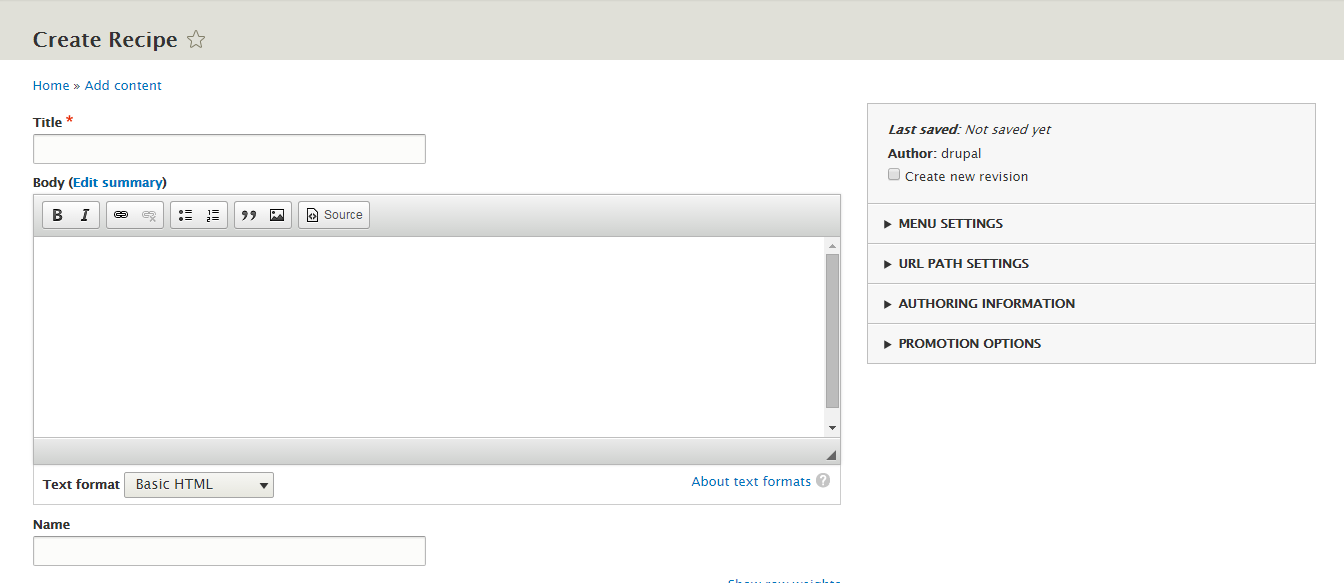
\includegraphics[width=\textwidth]{chapter5/bitingbugs_create_recipe_problem}
  	\caption{Create recipe form.}
  	\label{fig:bitingbugs_create_recipe_problem}
  \end{figure}
  
  \begin{figure}[H]
  	\centering
  	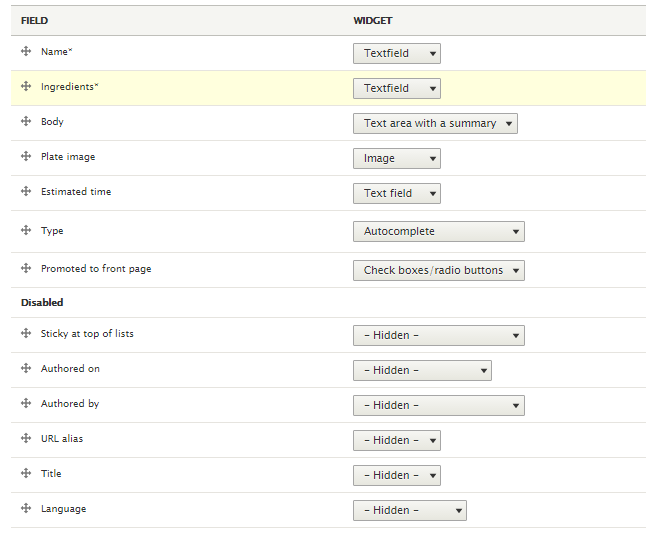
\includegraphics[width=\textwidth]{chapter5/bitingbugs_change_edit_display_recipe}
  	\caption{Manage recipe form display.}
  	\label{fig:bitingbugs_change_edit_display_recipe}
  \end{figure}
  
  Now go back to the content creation page: \textbf{Content $\rightarrow$ Add content $\rightarrow$ Recipe}. Use the following information:
  
  \begin{description}
  	\item[Name] Dry Roasted Crickets
  	\item[Ingredients] 25 – 50 live crickets
  	\item[Body] See file \url{recipe_roasted_crickets.txt}
  	\item[Image] See file \url{roasted_crickets.jpg}
  	\item[Alternative text] Plate of bugs
  	\item[Estimated time] 10
  	\item[Type] snack
  \end{description}
  
  Click \textbf{Save and publish}. You should see a page like figure \ref{fig:bitingbugs_roasted_crickets_recipe}.
  
  \begin{figure}[H]
  	\centering
  	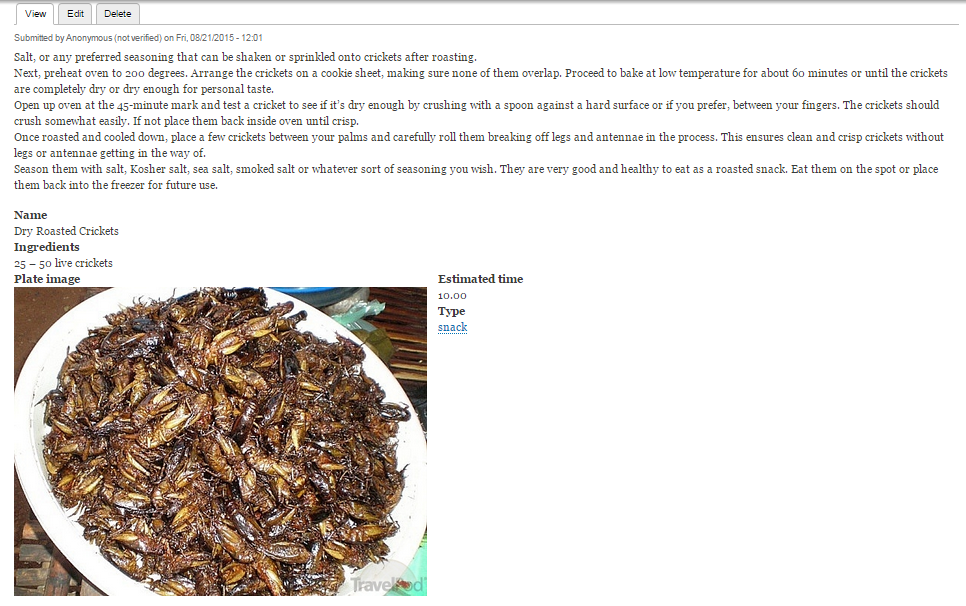
\includegraphics[width=\textwidth]{chapter5/bitingbugs_roasted_crickets_recipe}
  	\caption{Roasted crickets recipe.}
  	\label{fig:bitingbugs_roasted_crickets_recipe}
  \end{figure}
  
  We would like to change the way that our recipe is displayed. To do this go to: \textbf{Structure $\rightarrow$ Content types $\rightarrow$ Recipe $\rightarrow$ Manage display}. Change it to look like figure \ref{fig:bitingbugs_recipe_manage_display}
 
  \begin{figure}[H]
  	\centering
  	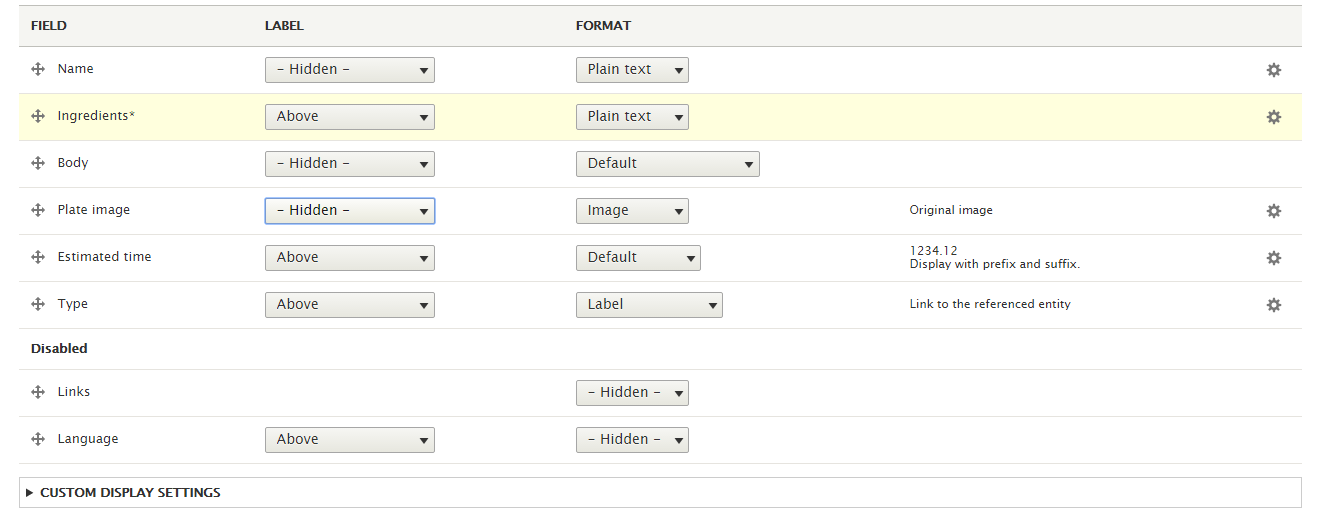
\includegraphics[width=\textwidth]{chapter5/bitingbugs_recipe_manage_display}
  	\caption{Manage recipe display}
  	\label{fig:bitingbugs_recipe_manage_display}
  \end{figure}
  
  Click \textbf{Save}. The new recipe page should look like figure \ref{fig:bitingbugs_roasted_crickets_recipe_updated}
  
  \begin{figure}[H]
  	\centering
  	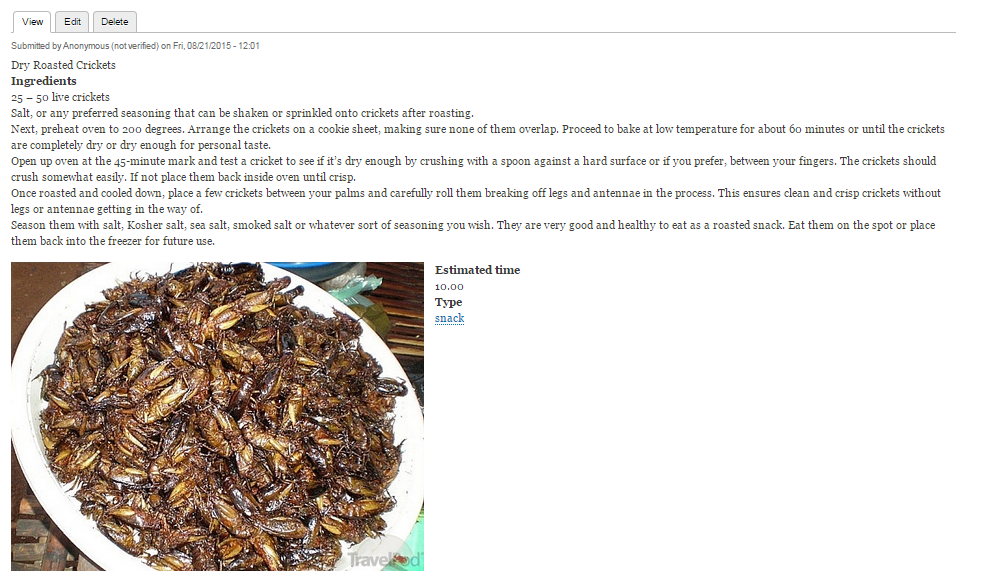
\includegraphics[width=\textwidth]{chapter5/bitingbugs_roasted_crickets_recipe_updated}
  	\caption{Recipe roasted crickets}
  	\label{fig:bitingbugs_roasted_crickets_recipe_updated}
  \end{figure}
  
  To be honest, is looks a bit better than before but still not great. In the chapter about theming we will learn how to further change the layout by adding custom css.
  
  \section{Review exercises}
  
  \begin{enumerate}
  	\item Go to the homepage of the Biting Bugs site. You should see a summary of the recipe we added earlier in this chapter (Figure \ref{fig:bitingbugs_recipe_homepage_summary}).  
  	
   \begin{figure}[H]
   	\centering
   	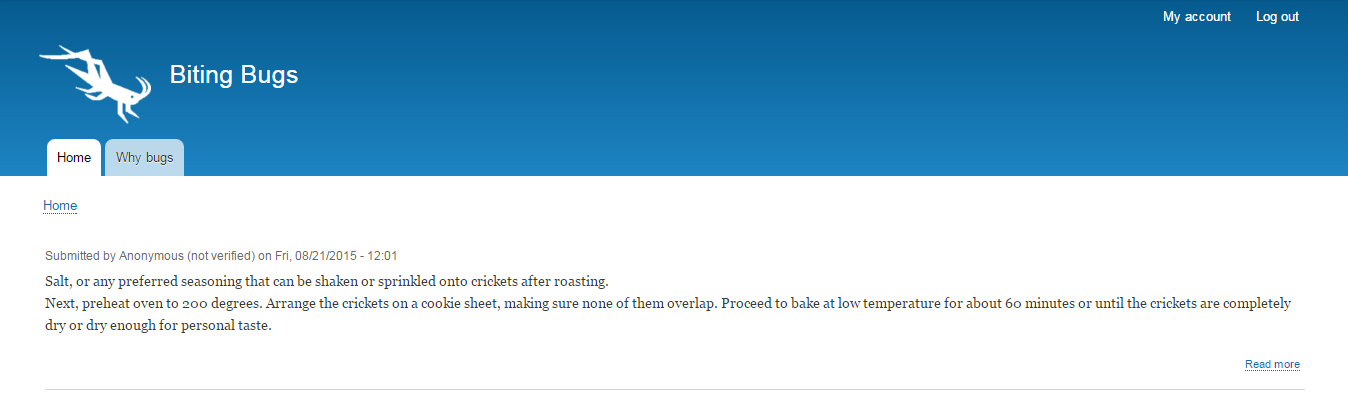
\includegraphics[width=\textwidth]{chapter5/bitingbugs_recipe_homepage_summary}
   	\caption{Recipe teaser}
   	\label{fig:bitingbugs_recipe_homepage_summary}
   \end{figure}
   
   Change the display settings of the recipe content type teaser display mode so it looks like figure \ref{fig:bitingbugs_recipe_homepage_summary_updated}. Make sure that when you click the image you go to the full recipe.
   
   \begin{figure}[H]
   	\centering
   	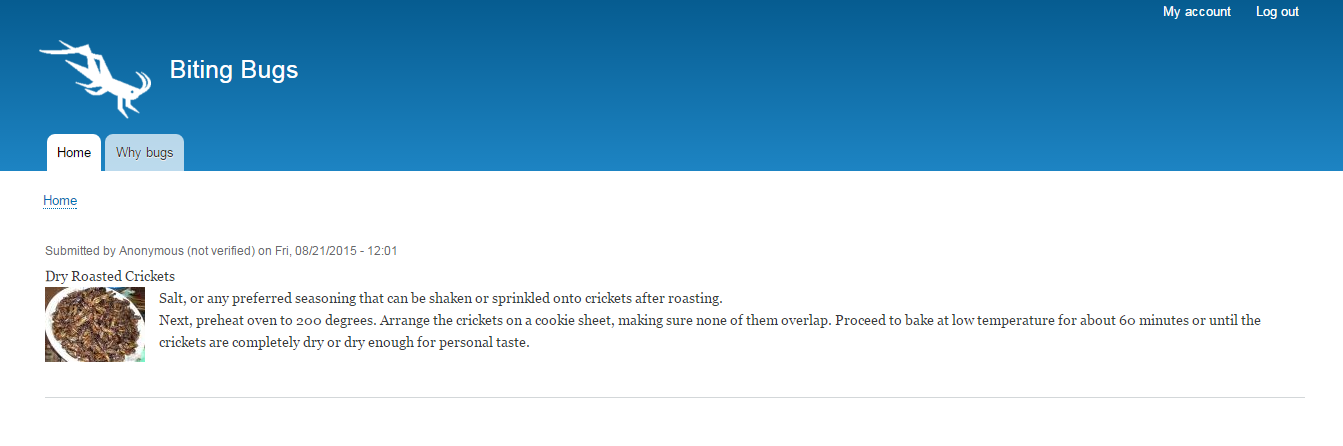
\includegraphics[width=\textwidth]{chapter5/bitingbugs_recipe_homepage_summary_updated}
   	\caption{Recipe teaser updated.}
   	\label{fig:bitingbugs_recipe_homepage_summary_updated}
   \end{figure}
   
   HINT: You can edit the image size by clicking on the gear next to the image field.
   
   \item Add three recipes to the bitingbugs site. You can find the recipes in the file \url{chapter5/recipes_with_bugs.txt}. Use the images: \url{cricket-flour.jpg}, \url{cricket_fried_rice.jpg} and \url{cricket_pad_thai.jpg}.
   
   \item Logout of the bitingbugs site. On the homepage you can see a login form on the left side of the page. Make sure the login form does not appear on the homepage. (HINT: after removing the login form from the homepage you can always login by going to \textbf{site hostname}/user for example  \url{bitingbugs.dd:8083/user})
   
   \item Change the display settings for the recipe teaser title so it links to the content.
   
   \item Change the Recipe content type so the author information is not displayed.
   
   \item Add a new basic page to the main menu. The basic page contains the information found in file \url{chapter5/edible_bugs.txt} and has the title \textbf{Edible bugs}. (Put the bug names in bold font.)
   
  \end{enumerate}